\documentclass[11pt,a4paper]{article}
\usepackage[margin=25mm]{geometry}
\usepackage[T1]{fontenc}
\usepackage[utf8]{inputenc}
\usepackage{lmodern}
\usepackage{xcolor}
\usepackage{hyperref}
\usepackage{graphicx}
\usepackage{parskip}
\definecolor{ink}{HTML}{17324D}
\definecolor{accent}{HTML}{087E8B}
\definecolor{gray}{HTML}{666666}
\hypersetup{colorlinks=true,urlcolor=accent}
\setlength{\parindent}{0pt}
\newcommand{\answerlines}[1]{\vspace{#1}\par\noindent\rule{\linewidth}{0.4pt}\par\vspace{3mm}\noindent\rule{\linewidth}{0.4pt}}
\begin{document}
\begin{center}
{\LARGE\bfseries\color{ink} IMU-Based Gesture Recognition}\\[2mm]
{\large Mini Project Topic Registration -- Embedded Systems 2026}\\[6mm]
\textbf{Name:} Matteo d'Amato\hspace{8mm}
\textbf{Email:} \href{mailto:mdamato@student.ethz.ch}{mdamato@student.ethz.ch}
\end{center}
\vspace{5mm}
\section*{Project Introduction}
This project will use the board's on-board IMU to analyze and classify motion gestures. I plan to recognize at least four gestures, with the option to add two more.
\begin{center}
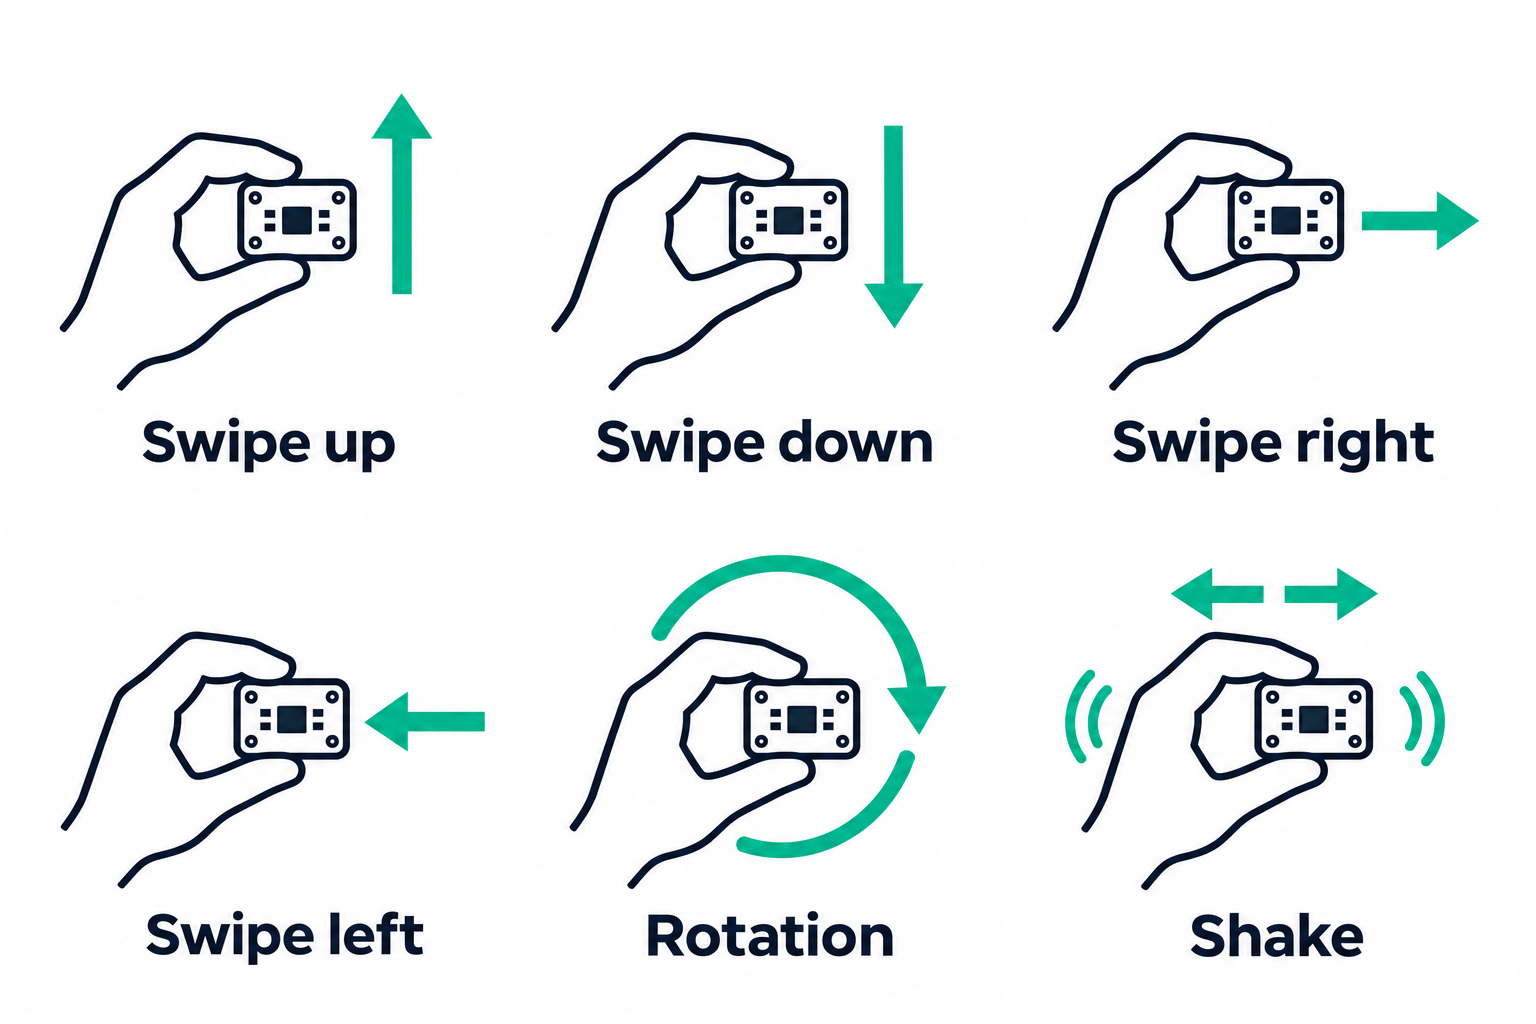
\includegraphics[width=0.65\linewidth]{gestures.png}
\end{center}


\section*{Motivation and Use Case}
Gesture recognition can support a wide range of applications. For this project, I plan to develop an accessibility tool for air writing. Each letter of the alphabet will be mapped to a sequence of gestures, allowing the STM32 board to act as a keyboard input device for a PC.  

The same system could also be adapted for other uses, such as controlling a PC cursor, a game, or presentation slides.


\section*{System Overview}
The gesture recognition tool will use the IMU integrated into the test board. I will first compare two different IMU data-processing algorithms and observe how their outputs differ. I will then use a threshold-based algorithm to classify the gestures. If time permits, I will also implement a small neural network and compare its performance with the threshold-based approach. 


\section*{Energy and Sleep-Mode Plan}
During normal operation, the STM32 will read and process IMU data while waiting for gestures. If no significant motion is detected for a defined period, the board will enter a low-power sleep mode. New IMU activity will wake the board and resume gesture recognition. I plan to compare energy use in active and sleep modes by measuring or estimating the current consumption and the time spent in each mode
\end{document}
